\section{Multi-Document Summarization}
In den letzten Jahren erzielten unterschiedliche Verfahren große Fortschritte beim automatisierten Zusammenfassen von mehreren Dokumenten zu einem repräsentativen Dokument.
Im Gegensatz zum normalen Zusammenfassen von einzelnen Dokumenten enthalten beim Multi-Document Zusammenfassen mehrere Dokumente über ein Thema viele redundante Informationen, die so gefiltert werden müssen, dass redundante Informationen nur einmal im Ausgabedokument dargestellt werden.
Ebenfalls ist das Verarbeiten von widersprüchlichen Informationen eine große Herausforderung bei der Zusammenfassung von mehreren Dokumenten.
Das Ziel von Multi-Document Summarization ist das zusammengefasste Repräsentieren der wichtigen Aspekte aller Dokumente in einem einzelnen Dokument, um einen guten allgemeinen Überblick zu schaffen.

Im weiteren Verlauf werden Multi-Document Summarization Systeme zur Zusammenfassung von Bewertungen verwendet.
Sei $R= \{x_i \}$ ein Datensatz von Bewertungen mit einzelnen Bewertungen $x=(x_1,...,x_{\| x \|})$ die aus einer Sequenz aus Wörtern bestehen.
Ziel ist es für ein gegebenes Produkt $p$ und die entsprechenden Bewertungen $R_p \subseteq R$ eine Zusammenfassung $s_p$ zu generieren, die alle relevanten Informationen faktisch korrekt representiert.


Insbesondere im Bereich der Multi-Review Summarization existieren viele unterschiedliche Ansätze.
Zum einen existieren extraktive Ansätze, wie zum Beispiel LexRank, ein unüberwachter Algorithmus der repräsentative Sätze für eine Bewertung basierend auf Ihrer Zentralität in einem TF-IDF gewichteten Graphen selektiert.
Zum anderen existieren abstraktive Ansätze wie zum Beispiel MeanSum, CopyCat oder COOP, die generative Ansätze verwenden um neuartige Sätze in den Bewertungen zu erzeugen.

Die abstraktiven Modelle basieren auf Autoencoder Architekturen. Es wird ein Encoder $E_\phi : X \rightarrow Z$ verwendet, um Textrepräsentationen in einen Latentvektor im Latentraum $Z$ umzuwandeln.
Aus den Latentvektoren $z$ kann anschließend unter Verwendung von einem Decoder $D_\theta : Z \rightarrow \hat{X}$ eine Textrepräsentation generiert werden.


MeanSum ist ein Autoencoder Modell mit LSTM Encoder und Decoder und errechnet zur Zusammenfassung von Bewertungen den Durchschnitt von den einzelnen Latentvektoren der Bewertungen $z_p = \bar{z} \text{, mit } z=\{z_{p_1},z_{p_2},...z_{p_k}\}$.
Von diesem Durchschnittslatentvektor $z_p$ wird anschließend eine Bewertung generiert. 


CopyCat basiert auf einem Variational Autoencoder Modell, welches GRU Encoder und Decoder verwendet. 
Für jede Gruppe von Bewertungen berechnet CopyCat einen Latentvektor $c$ der die gesamte Semantik der Gruppe beschreibt. 
Weiterhin wird jede einzelne Bewertung einer Gruppe mit einem einzelnen Latentvektor $z$ beschrieben.
Bei der Generation von Durchschnittsbewertungen ermöglicht es CopyCat dem Decoder, die einzelnen Latentvektoren für die Bewertungen $z_i$, den allgemeinen Gruppenvektor $c$ und die Bewertungen $r_i$ an sich zu betrachten.
Durch den Zugriff auf die anderen Bewertungen $r_i$ kann der Decoder spezifische Worte von diesen \glqq kopieren\grqq{}  und somit übernehmen.



\subsection{Convex Aggregation for Opinion Summarization}
\label{coop}
Convex Aggregation for Opinion Summarization kurz COOP, ist eine Methode, die unterschiedliche Kombinationenen von einzelnen Latentvektoren zum Berechnen einer Durchschnittsbewertung untersucht.
Bei der Verwendung von Variational Autoencodern werden die einzelnen Eingabebewertungen durch einen Latentvektor repräsentiert. 
Häufig wird im nächsten Schritt zur Berechnung einer Durchschnittsbewertung, der normale Durchschnitt aller verwendeten Latentvektoren bestimmt und von diesem eine neue Durchschnittsbewertung generiert.

\begin{figure}[h]
    \centering
    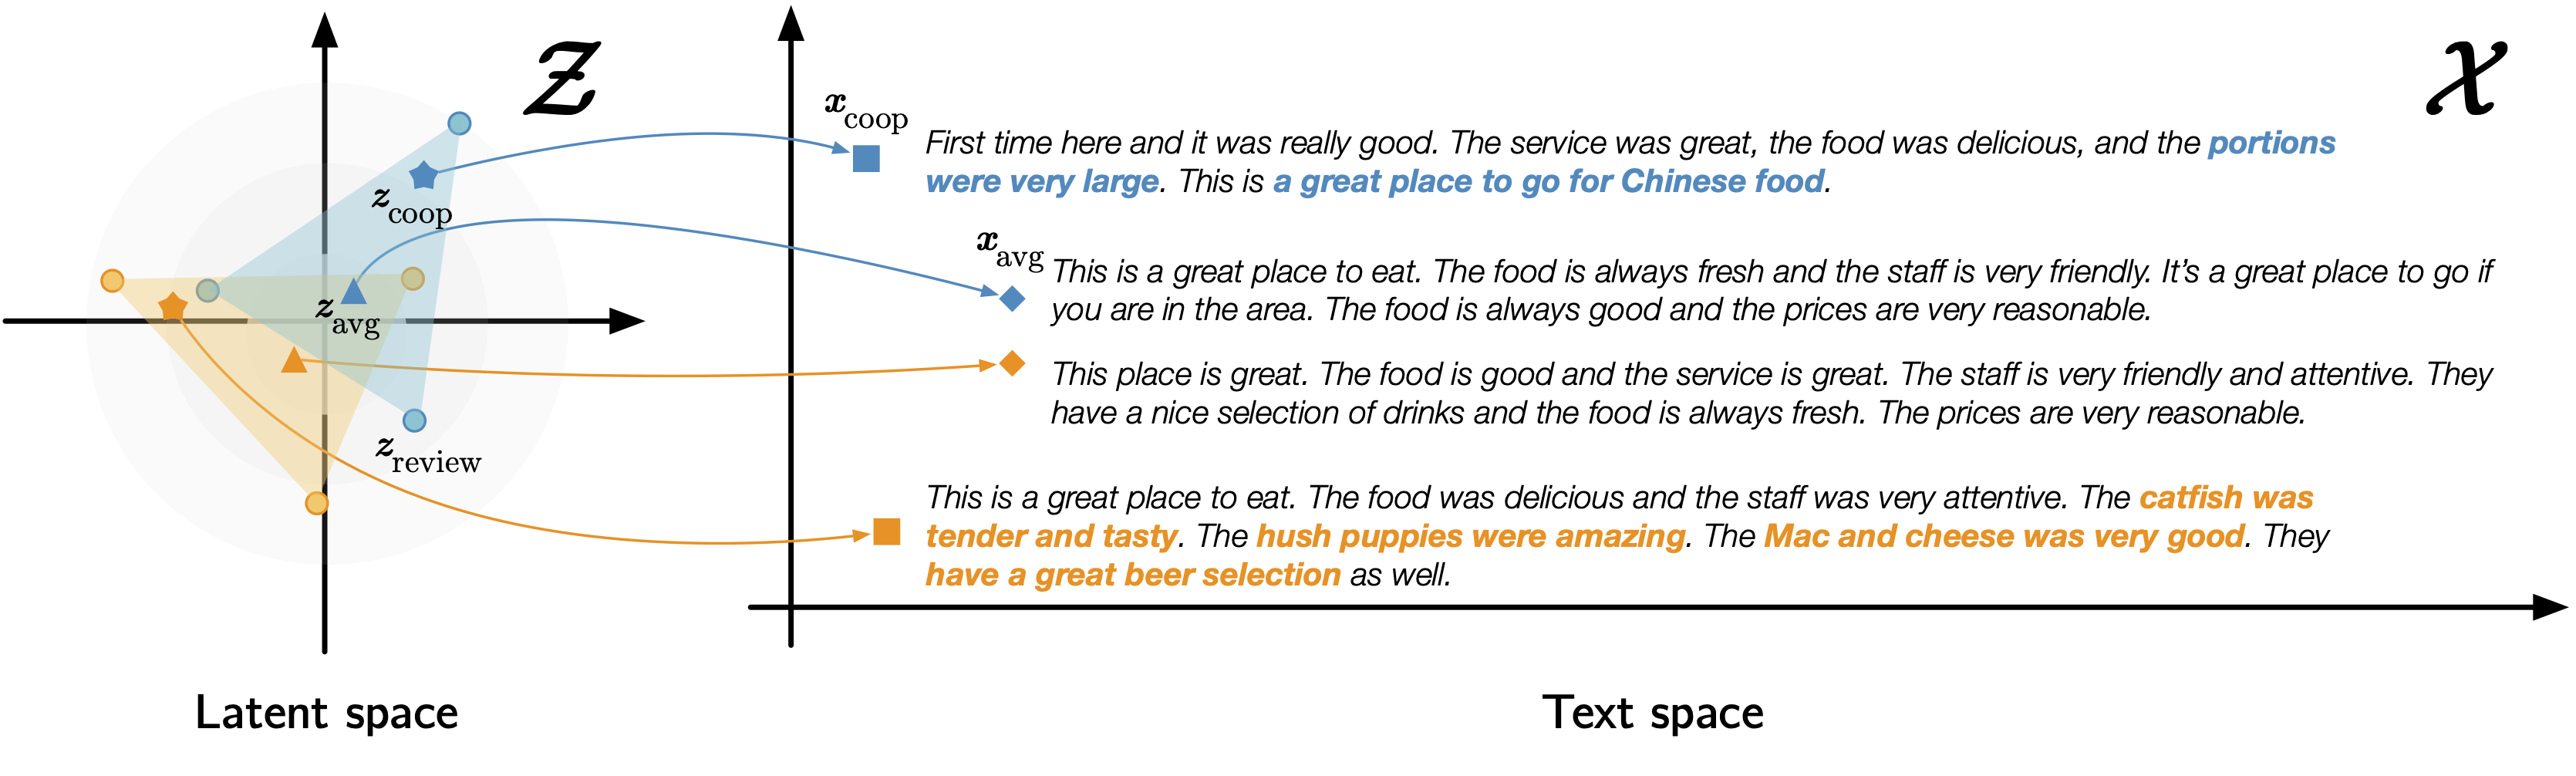
\includegraphics[width=\textwidth]{bilder/coop}
    \caption{Latentraum $Z$ mit den entsprechenden generierten Bewertungen $X$.}
    \label{coop_fig}
\end{figure}

Wie in Abbildung \ref{coop_fig} zu erkennen ist, ähneln sich Bewertungen die durch Bestimmung des Durchschnitts der Latentvektoren generiert worden sind sehr. 
Auffällig ist die Relation zwischen der Ausdrucksstärke und dem Informationsgehalt eines Latentvektors und seiner $L_2$-Norm $\| z \|$.
Latentvektoren die durch den Durschnitt bestimmt werden haben eine geringere $L_2$-Norm und somit in den erzeugten Bewertungen einen geringeren Informationsgehalt.

Um ausdrucksstarke Latentvektoren für die Generation der Bewertungen zu erhalten formuliert COOP die Bestimmung des optimalen Latentvektors als Optimierungsproblem, um die beste Kombination von einzelnen Latentvektoren zu finden.
\begin{alignat}{2}
    \max_z              &\quad&  Overlap(R_p, D_\theta(z))    & \\
    \text{unter der Nebenbedingung: } &\quad&  z = \sum_{i=1}^{|R_p|} w_i z_i \\
                         &\quad&  \sum_{i=1}^{|R_p|}w_i=1,                        &\quad \forall w_i \in \mathbb{R}^+
\end{alignat}
Optimiert wird das Maximieren des \textit{input-ouput-word overlap} zwischen den Eingabebewertungen $R_p$ und der generierten Bewertung $D_\theta(z)$. 
Diese \textit{Overlap}-Metrik basiert auf dem Rouge-1 F1 Score und ermöglicht es Bewertungen zu generieren die konsistent zu den Eingabebewertungen sind.
Die Suche der einzelnen Kombinationen wird auf die Potenzmenge der Eingabebewertungen $R_p$ beschränkt. 
Der Zusammenfassunslatentvektor $z_p$ wird anschließend aus dem Durchschnitt der ausgewählten Eingabebewertungslatentvektoren berechnet.
\begin{align}
z_p = \frac{1}{|R_p^{'}|} \sum_{i=1}^{R_p^{'}}z_i \text{ ,mit } R_p^{'} \in 2^{R_p} \setminus  \{ \emptyset\}
\end{align}
Die COOP Methode zur Kombination von den einzelnen Latentvektoren, um ausdrucksstarke Bewertungen zu erhalten, erreicht State-of-the-Art Ergebnisse im Vergleich zu anderen Methoden, die den normalen Durchschnittslatentvektor verwenden.
Die erzeugten Bewertungen sind gut repräsentativ für eine Gruppe von Bewertungen und erhalten ein hohes Maß an Informationen. 
Trotzdem stellt sich die Frage, ob und inwiefern sich diese Ergebnisse noch weiter optimieren lassen.
Im weiteren Verlauf wurde ein Verfahren entwickelt, welches entsprechende Latentvektoren weiterhin adaptiert, um ein noch höheres \textit{Input-Output-Overlapping} zu erhalten und somit präzisere Informationen in den Durchschnittsbewertungen zu generieren.

\pagebreak
